\chapter{Methods and techniques}%
\label{ch:methods}

The works described in~\autoref{ch:paper1}, \autoref{ch:paper2}, and
\autoref{ch:paper3} consist of contributions related to the computational
elucidation of reaction mechanisms.
As such, computational methods were used to investigate the mechanisms by
modelling the chemical reactions and comparing hypotheses to each other,
to the literature and to the available experimental data.

This chapter presents an account of the relevant computational methods and
techniques used in the works.
Basic background on computational chemistry is given in
\autoref{sec:background-methods}.
Details about the methods used in the development of the \overreact software
package are given in \autoref{sec:overreact-methods}.

\subimport{.}{methods/background}
\subimport{.}{methods/overreact}

\section{Chemical reaction mechanisms}

SOME OF THOSE THINGS MIGHT GO INTO THE METHODS.

\subsection{Bell-Evans-Polanyi principle}

The Bell-Evans-Polanyi (BEP) principle is a fundamental principle in the study
of chemical reactions.
It states that the more exothermic reactions usually have to overcome lower
reaction barriers and are therefore faster.

It is customary to successfully extend this concept to exergonic reactions.
But since the largest contribution is the electronic energy, it is reasonably
safe to apply the BEP principle (and Hammer's postulate, as we will see later)
using electronic energies in the context of quantum chemistry calculations.

CITATION.

\subsection{Hammond's postulate}

CITATION.

\subsection{Effects worth investigating}

\subsubsection{Some Pd and Pd chemistry}

\subsubsection{Organometallic chemistry}

\subsubsection{Organocatalysis}

\subsubsection{Outersphere effects}

\section{Intramolecular and substitutional effects: a key step to understand
enzyme-like catalysis}

Despite the great advancements in the developments of artificial enzymes~\cite{Breslow_1995},
the synthetic reproduction of the reaction rate accelerations attained by
natural enzymes is far from being reached.
To get there, we will need a more detailed comprehension of the ways enzymes
work at the molecular level~\cite{Catalysis_in_Chemistry_and_Enzymology}.
Much effort has been put in this direction, with at least six Nobel Prizes
awarded to this and related areas~\cite{Nobel_1929,Nobel_1946,Nobel_1957,Nobel_1975,Nobel_1997,Nobel_2013}.
These and other progresses show that the main source of acceleration in
enzymatic reactions is to be found in the events that accompany the
enzyme-substrate complex formation that leads to bond breaking and
formation~\cite{Catalysis_in_Chemistry_and_Enzymology}.
These events induce conformational changes in both substrate and enzyme, which
enhances the interactions in the active site~\cite{Fischer_1890,Fischer_1894,Koshland_1958,Dafforn_1971,Kirby_1996}.
As a result, substrate active centers adequately orient themselves towards
their counterparts in the active site, which leads to
i. a decrease in stability of the ground state (if compared with the
        free substrate state),
ii. a lowering of the transition state energy (if compared with the
        non-catalyzed reaction),
iii. energy relaxation through the formation of intermediates and
        products.

These driving forces are also found in intramolecular reactions (\autoref{fig:reacoes-intramoleculares}).
%
\begin{figure}[hbtp]
    \centering
    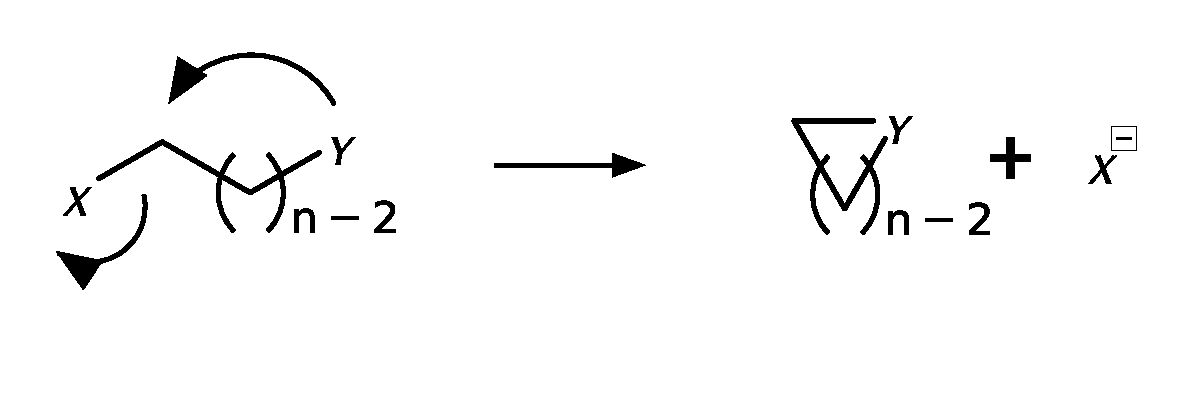
\includegraphics[width=.6\textwidth]{figures/reacao-intramolecular}
    \caption[Typical scheme of an intramolecular reactions]{
        Reaction scheme of a typical intramolecular reaction, whose products or
        intermediates are often cycles.
        Smaller rings ($n \le 4 $)
        tend to be disfavored by enthalpy, while larger rings ($n \ge 7 $)
        have less probable formation due to entropy.}%
    \label{fig:reacoes-intramoleculares}
\end{figure}
%
In fact, the similarities between monomolecular enzymatic processes and
intramolecular reactions have been already recognized~\cite{Nilsson_1933,Bruice_1960b,Jung_1990}.
Despite the limitations of using intramolecular reactions as a model for
enzymatic reactions, it is natural to suppose that the detailed understanding
of enzyme catalysis has, as a prerequisite, the ability to understand the
related processes in simpler systems.~\cite{Kirby_1972}.

We have studied some of these effects.

PAPER 1 => is peptide-like/enzyme-like? is intramolecular/substitutional?

PAPER 2 => is peptide-like/enzyme-like? is intramolecular/substitutional?

PAPER 3 => is peptide-like/enzyme-like? is intramolecular/substitutional?
=> \emph{\ce{N}}-alkyl substituted maleamic acids
Particular details concerning the intramolecular effects of geminal and
vicinal disubstitutions can be found in \autoref{ch:gem-vic-disubstitions}.
